\documentclass[../Main.tex]{subfiles}

\begin{document}
    \subsection{Overview}
        As I am creating a game, it must be designed with that in mind. Therefore, most parts of the game will be stored in classes, with a couple of singletons designed with doing the key aspects of the game, e.g. managing the application, rendering the game, and logging warnings or messages so that it is easier to debug errors. Furthermore, the game must be able to be compiled for both Linux and Windows as I use both Linux and Windows. Finally when developing the game, it will be compiled with some features that will allow me to alter settings while inside the game, which will allow for faster development.

        Furthermore, during my development of the project I shall need to use some packages to allow me to more easily create the game, without having to program every little part of the game, the packages I will be using are:
        \begin{itemize}
            \item FreeType - This is used to make text rendering easier.
            \item GLEW and GLFW - These are used so as an OpenGL implementation I can use to render objects on the screen.
            \item ImGui - This is used for when debugging - and is not compiled in the release version. It allows for me to have a simple menu which I can program to change variables or call functions when th program is running.
            \item GLM - This is a simple library designed for OpenGL. It has a few utils that are easy to use and are extremely optimised.
            \item stb\_image - This is for loading images into the game for textures.
        \end{itemize}

    \subsection{Maze Generation}
        \subsubsection{Storage}
            I have developed a special method of storing the rooms in the maze, to start off, it will be stored in a 1d array (which acts like a 2d array when getting rooms, using coordinates), then when generating more of the maze, when the player moves, 2 variables will be altered storing the offset of the x and y coordinates - which will allow the maze to not move and reallocate all the rooms stored.

            Instead imagine when storing a room at position (0, 0) or index 0 in the array. When the maze needs to generate more of the maze on the north, the position in the array of that room will not change, it will still be at index 0, however the coordinates will change as its moved down therefore its now at (0, -1), and the new rooms generated will be at the end of the maze. However when accessing the array with the coordinate system it will seem as though all the rooms have moved down 1. This will save processing power moving all the rooms to different indices in the array.

            However, the rooms also will have to store coordinates of where they are. This results in having to go through all the rooms and updating the coordinates. To reduce this as much as possible, the coordinates will only be updates when one of the offsets loops back to the center, so for example going back to 0.

        \clearpage
        \subsubsection{Prototype}
        For a prototype of the generation, I decided to write it in python with a room just consisting of being a cross section, this was to make sure that it wasn't too complex, while keeping the basic idea of the generation.
        \begin{figure}[hbt!]
            \centerline{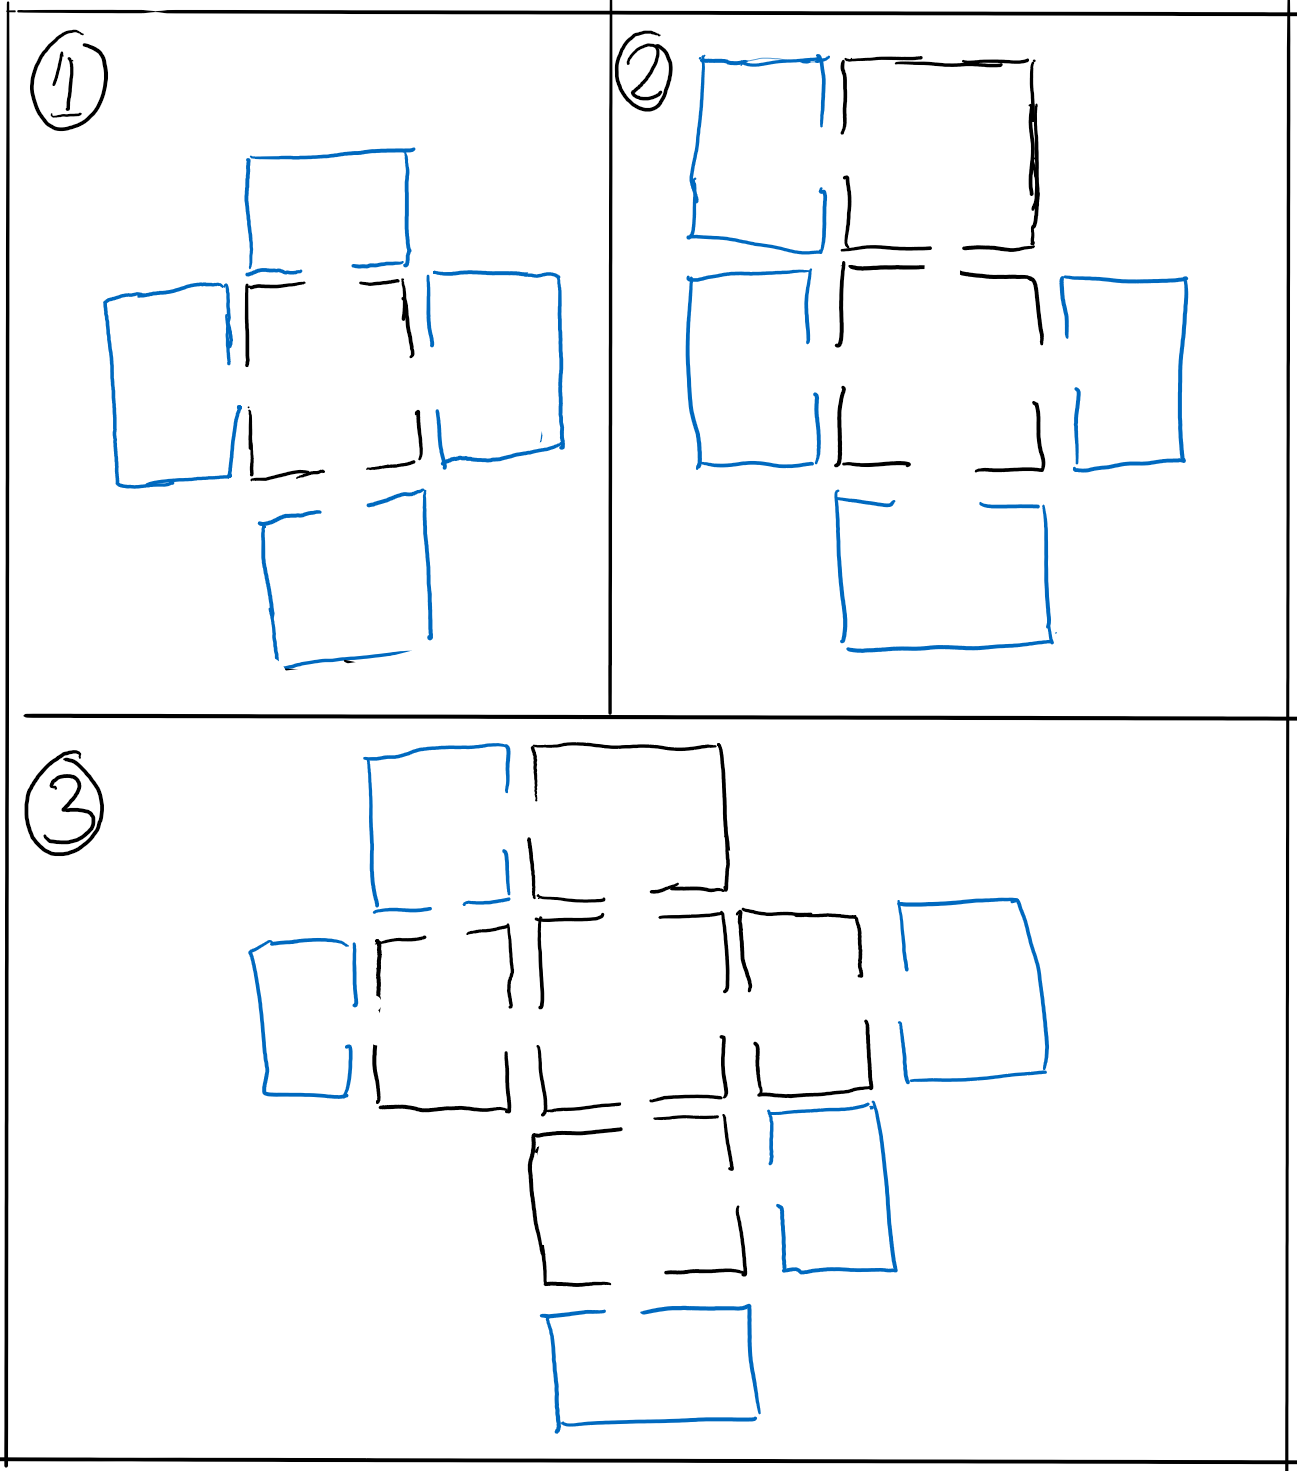
\includegraphics[scale=0.5]{img/Design/Maze Generation.png}}
            \caption{Steps followed by the maze generation}
            \label{fig:MazeGen}
        \end{figure}

        The figure above briefly shows planning behind how the maze generation works, with the rooms outlined in black, as rooms that have a set place, with then the rooms highlighted in blue being the rooms yet to be generated, and thus in the "current" list.

        \clearpage
        \lstinputlisting[language = Python]{prototypes/MazeGen.py}

        \clearpage
        \begin{multicols*}{3}
            [
                \subsubsection{Output}
                This is the output of the prototype, with the 'X' representing a wall and blank space represented as path the player can walk through. I have also shown the output of the maze when the player moves south and east. The new sections of the maze generated, after taking each step, is highlighted in yellow.
            ]
            The first output \par
            \centerline{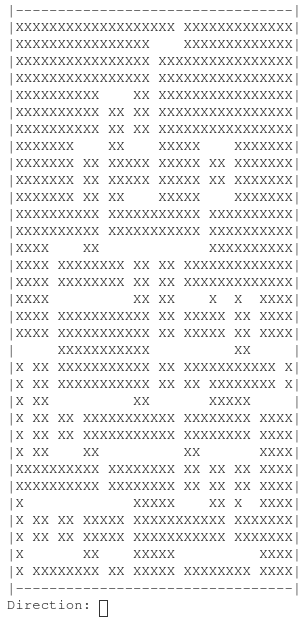
\includegraphics[width=0.8\linewidth]{img/Design/Output1.png}}

            \columnbreak
            After moving south (downwards) \par
            \centerline{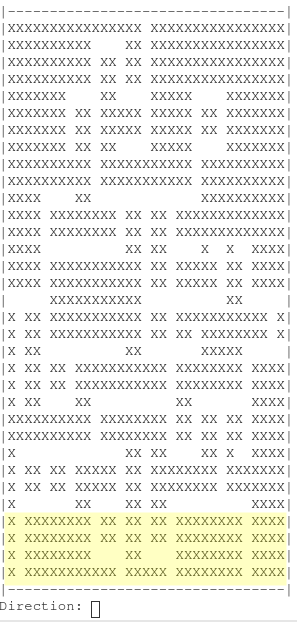
\includegraphics[width=0.75\linewidth]{img/Design/Output2.png}}


            \columnbreak
            After moving east (leftwards) \par
            \centerline{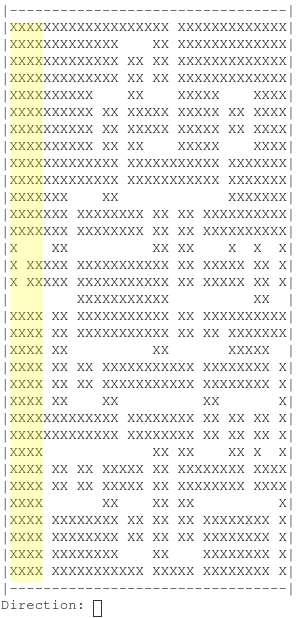
\includegraphics[width=0.8\linewidth]{img/Design/Output3.png}}
        \end{multicols*}

    \subsection{A* Algorithm}
        \subsubsection{Explanation}
            This is a common algorithm used for finding the shortest route between two points because speed while also being very versatile.
            \begin{figure}[hbt!]
                \centerline{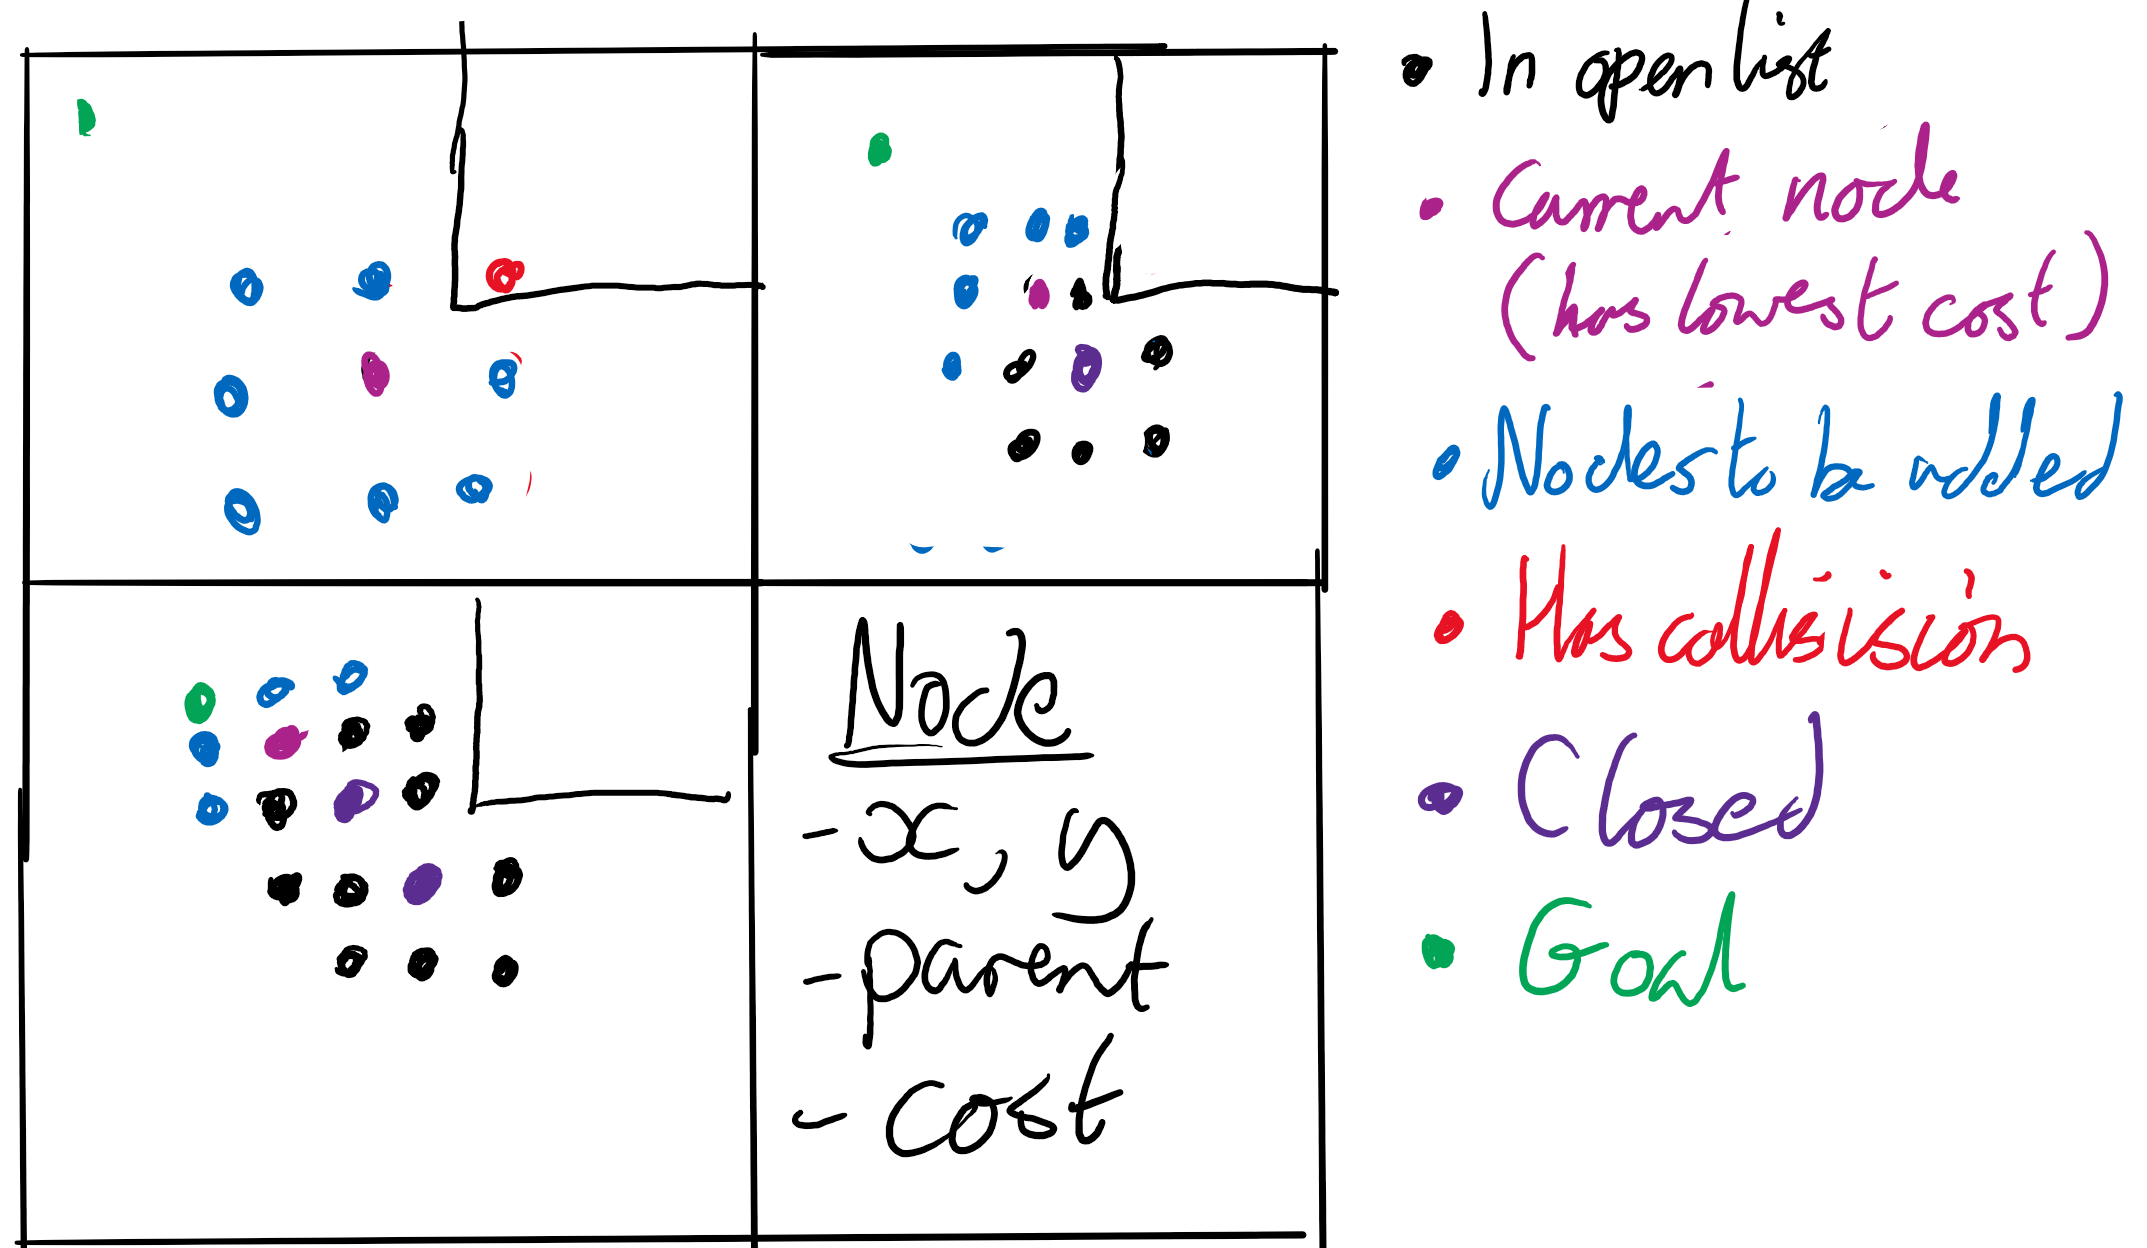
\includegraphics[scale=0.3]{img/Design/A-star algorithm.png}}
                \caption{Drawing describing the process of how the A* algorithm finds the shortest route}
                \label{fig:AStar}
            \end{figure}

            The final box shows what the Node class needs to store, in order for this to work, with the different colours representing different states a node can be in, labelled on the side.
        \subsubsection{Prototype} % TODO: Write a prototype
            To test the plan behind the A* algorithm I decided to make a version in Python with a set maze, which I can then input different coordinates to see if it works efficiently. From running the program, this version seemed to be extremely fast, even in Python.
            \lstinputlisting[language = Python]{prototypes/AStar.py}
        \begin{multicols*}{3}
            [
                \subsubsection{Output}
                This is the output of the A* algorithm, given 3 different coordinates to work towards. The 'X' represent solid walls and the green 'O' represent the path produced by the algorithm.
            ]
            First test: From (1, 1) to (3, 1) \par
            \centerline{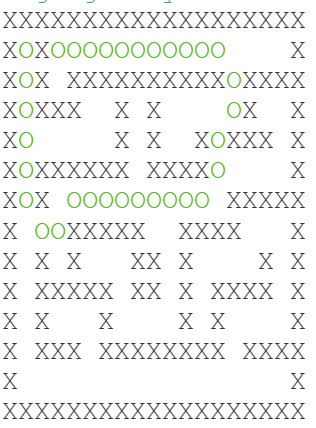
\includegraphics[width=0.8\linewidth]{img/Design/AStarPrototype1.png}}

            \columnbreak
            Second test: From (1, 1) to (17, 12) \par
            \centerline{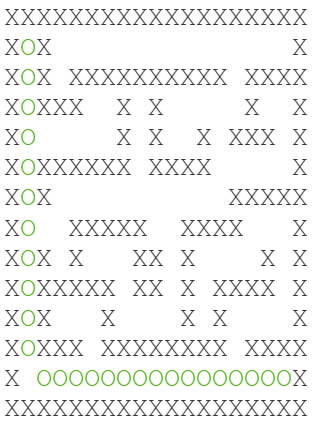
\includegraphics[width=0.75\linewidth]{img/Design/AStarPrototype2.png}}


            \columnbreak
            Third test: From (1, 1) to (12, 10) \par
            \centerline{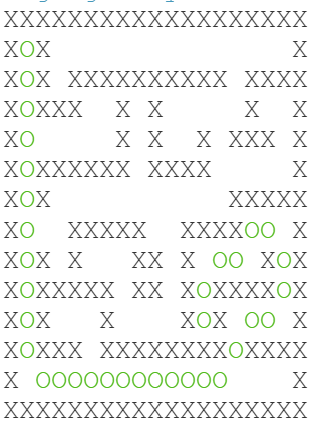
\includegraphics[width=0.8\linewidth]{img/Design/AStarPrototype3.png}}
        \end{multicols*}

    \clearpage
    \subsection{Graphical Design}
        \subsubsection{Overall Design}
            The overall design is (as shown below) to have a simple GUI system where the player can see what current weapons they have available to them as well as their health, then a simple button at the top to pause the game and go back to a menu screen. Furthermore, the camera will be facing downwards and is above the player. This will make it easier to create a rendering system and allows the player to explore in any direction (except up and down). Items will be able to be found on the ground, with rendered with their texture, and not a back or anything to allow anyone to easily discern between the different objects.

            Each room will be simple, with different objects in the center, for example this room has a chest in the center which the player will be able to interact with and grab items out of. Then there can be entrances at the top, bottom, left and right of the room and will be generated using the method talked above (in the maze generation section).
            \begin{figure}[hbt!]
                \centerline{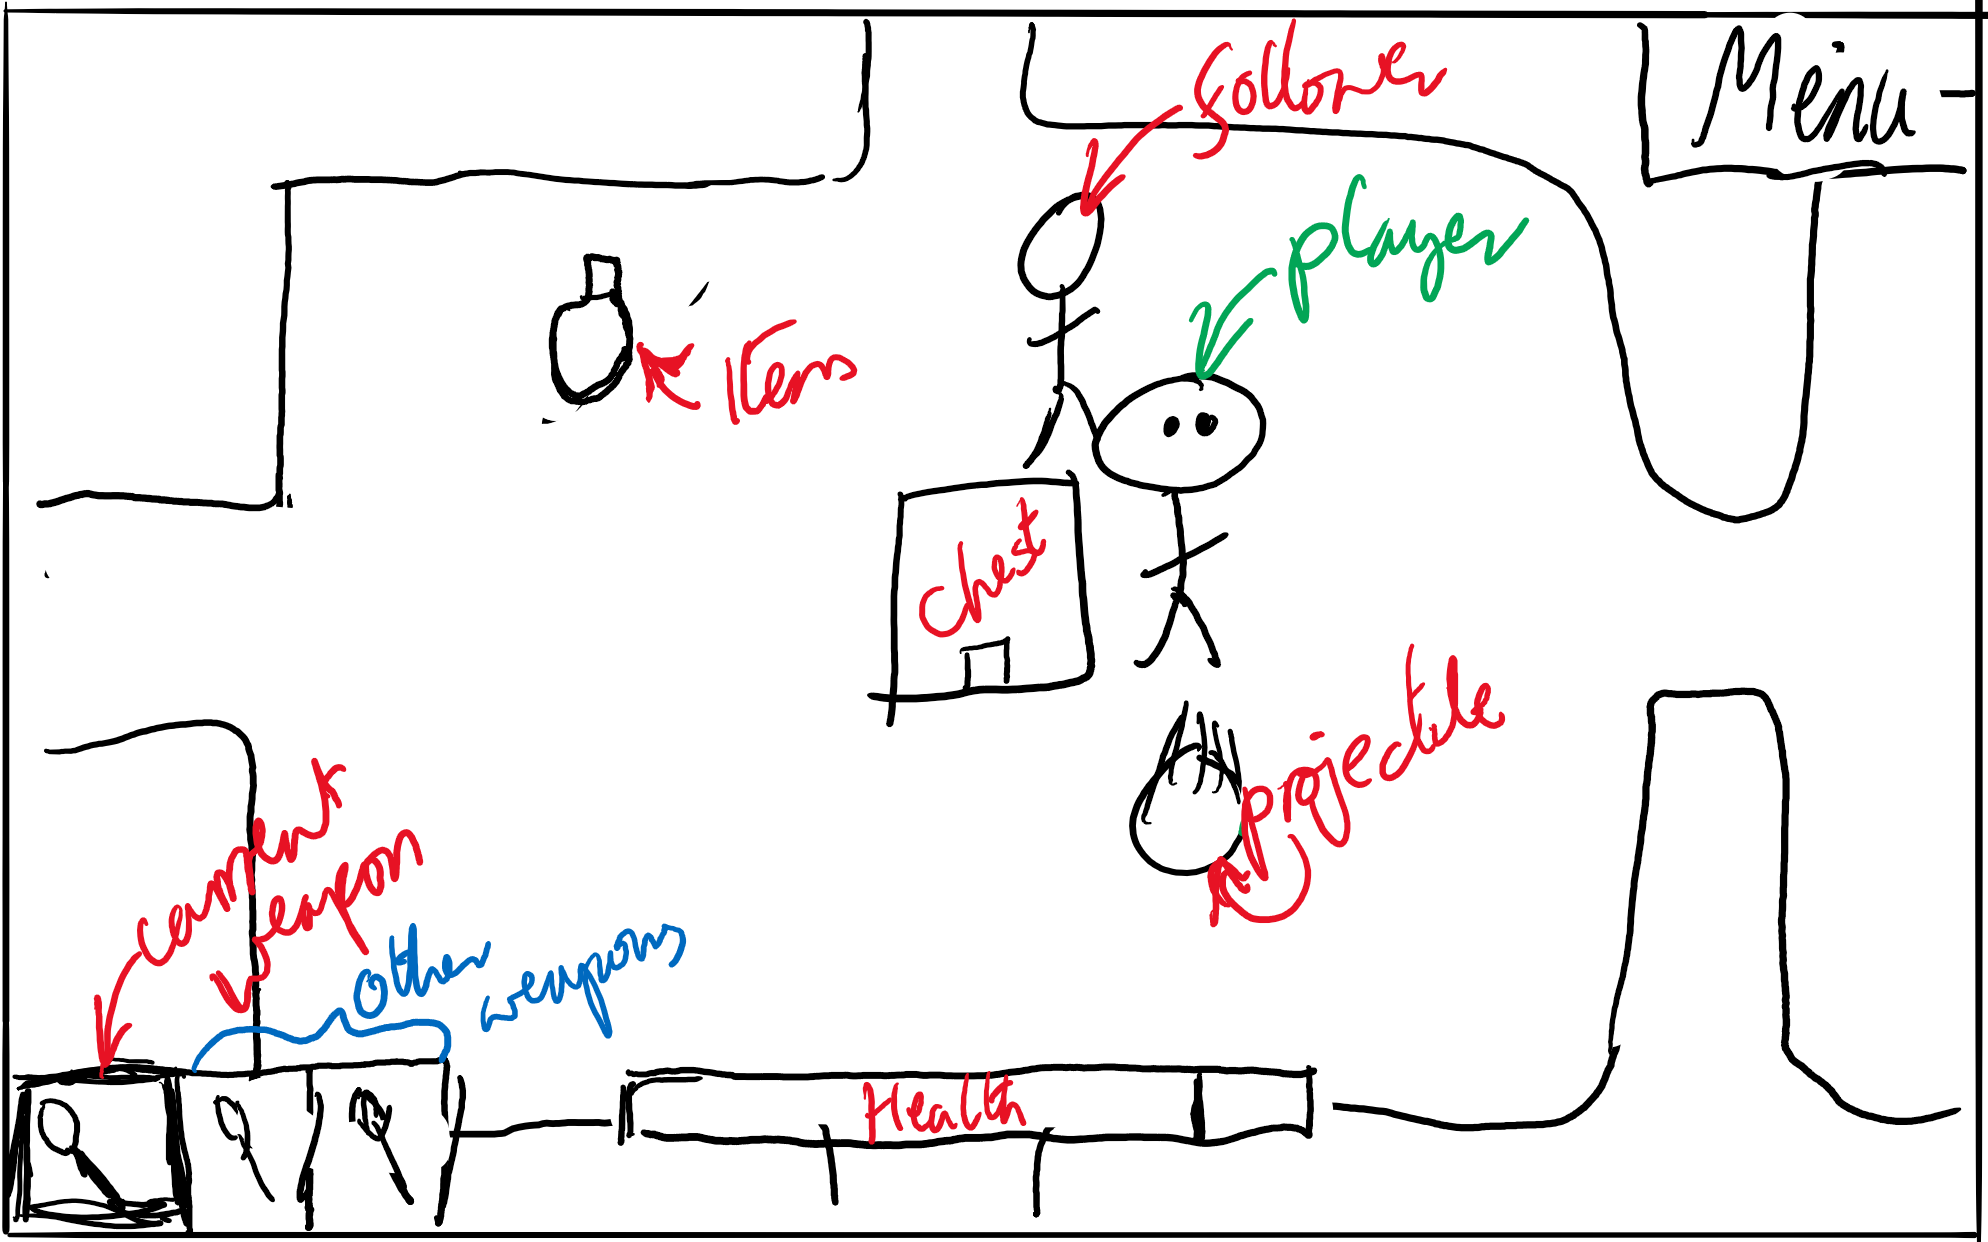
\includegraphics[scale=0.3]{img/Design/Overall Design.png}}
                \caption{Overall Design plan}
                \label{fig:OverallDesign}
            \end{figure}

            Please note that the weapons, potions, and books were gained from Shikashi's Fantasy Icons Pack v2 by Matt Firth. Also the tiles for the rooms were altered slightly to fit the needed tiles however the textures were originally from RPG Nature Tileset - Seasons by Stealthix. However, I will be making the design for each of the npcs as I cannot find any that will fit the design.

        \clearpage
        \subsubsection{NPCs}
            \begin{center}
                \begin{tabular}{ | m{0.13\textwidth} | m{0.11\textwidth} m{0.12\textwidth} m{0.12\textwidth} m{0.12\textwidth} m{0.12\textwidth} m{0.12\textwidth} | }
                    \hline
                    \textbf{Name} & & & & & & \\
                    \hline
                    \multirow{2}{*}{\textbf{Player}} & \centerline{
\includegraphics[scale=3]{../res/textures/entities/player/heir/North.png}} & \centerline{
\includegraphics[scale=3]{../res/textures/entities/player/heir/North-Walk-1.png}} & \centerline{
\includegraphics[scale=3]{../res/textures/entities/player/heir/North-Walk-2.png}} & \centerline{
\includegraphics[scale=3]{../res/textures/entities/player/heir/South.png}} & \centerline{
\includegraphics[scale=3]{../res/textures/entities/player/heir/South-Walk-1.png}} & \centerline{
\includegraphics[scale=3]{../res/textures/entities/player/heir/South-Walk-2.png}} \\
                    & \centerline{
\includegraphics[scale=3]{../res/textures/entities/player/heir/East.png}} & \centerline{
\includegraphics[scale=3]{../res/textures/entities/player/heir/East-Walk-1.png}} & \centerline{
\includegraphics[scale=3]{../res/textures/entities/player/heir/East-Walk-2.png}} & \centerline{
\includegraphics[scale=3]{../res/textures/entities/player/heir/West.png}} & \centerline{
\includegraphics[scale=3]{../res/textures/entities/player/heir/West-Walk-1.png}} & \centerline{
\includegraphics[scale=3]{../res/textures/entities/player/heir/West-Walk-2.png}} \\
                    \hline
                    \multirow{2}{*}{\textbf{FrostFollower}} & \centerline{
\includegraphics[scale=3]{../res/textures/entities/followers/frost/North.png}} & \centerline{
\includegraphics[scale=3]{../res/textures/entities/followers/frost/North-Walk-1.png}} & \centerline{
\includegraphics[scale=3]{../res/textures/entities/followers/frost/North-Walk-2.png}} & \centerline{
\includegraphics[scale=3]{../res/textures/entities/followers/frost/South.png}} & \centerline{
\includegraphics[scale=3]{../res/textures/entities/followers/frost/South-Walk-1.png}} & \centerline{
\includegraphics[scale=3]{../res/textures/entities/followers/frost/South-Walk-2.png}} \\
                    & \centerline{
\includegraphics[scale=3]{../res/textures/entities/followers/frost/East.png}} & \centerline{
\includegraphics[scale=3]{../res/textures/entities/followers/frost/East-Walk-1.png}} & \centerline{
\includegraphics[scale=3]{../res/textures/entities/followers/frost/East-Walk-2.png}} & \centerline{
\includegraphics[scale=3]{../res/textures/entities/followers/frost/West.png}} & \centerline{
\includegraphics[scale=3]{../res/textures/entities/followers/frost/West-Walk-1.png}} & \centerline{
\includegraphics[scale=3]{../res/textures/entities/followers/frost/West-Walk-2.png}} \\
                    \hline
                    \multirow{2}{*}{\textbf{FireFollower}} & \centerline{
\includegraphics[scale=3]{../res/textures/entities/followers/fire/North.png}} & \centerline{
\includegraphics[scale=3]{../res/textures/entities/followers/fire/North-Walk-1.png}} & \centerline{
\includegraphics[scale=3]{../res/textures/entities/followers/fire/North-Walk-2.png}} & \centerline{
\includegraphics[scale=3]{../res/textures/entities/followers/fire/South.png}} & \centerline{
\includegraphics[scale=3]{../res/textures/entities/followers/fire/South-Walk-1.png}} & \centerline{
\includegraphics[scale=3]{../res/textures/entities/followers/fire/South-Walk-2.png}} \\
                    & \centerline{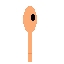
\includegraphics[scale=3]{../res/textures/entities/followers/fire/East.png}} & \centerline{
\includegraphics[scale=3]{../res/textures/entities/followers/fire/East-Walk-1.png}} & \centerline{
\includegraphics[scale=3]{../res/textures/entities/followers/fire/East-Walk-2.png}} & \centerline{
\includegraphics[scale=3]{../res/textures/entities/followers/fire/West.png}} & \centerline{
\includegraphics[scale=3]{../res/textures/entities/followers/fire/West-Walk-1.png}} & \centerline{
\includegraphics[scale=3]{../res/textures/entities/followers/fire/West-Walk-2.png}} \\
                    \hline
                    \multirow{2}{*}{\textbf{DarkFollower}} & \centerline{
\includegraphics[scale=3]{../res/textures/entities/followers/dark/North.png}} & \centerline{
\includegraphics[scale=3]{../res/textures/entities/followers/dark/North-Walk-1.png}} & \centerline{
\includegraphics[scale=3]{../res/textures/entities/followers/dark/North-Walk-2.png}} & \centerline{
\includegraphics[scale=3]{../res/textures/entities/followers/dark/South.png}} & \centerline{
\includegraphics[scale=3]{../res/textures/entities/followers/dark/South-Walk-1.png}} & \centerline{\includegraphics[scale=3]{../res/textures/entities/followers/dark/South-Walk-2.png}} \\
                    & \centerline{\includegraphics[scale=3]{../res/textures/entities/followers/dark/East.png}} & \centerline{\includegraphics[scale=3]{../res/textures/entities/followers/dark/East-Walk-1.png}} & \centerline{\includegraphics[scale=3]{../res/textures/entities/followers/dark/East-Walk-2.png}} & \centerline{\includegraphics[scale=3]{../res/textures/entities/followers/dark/West.png}} & \centerline{\includegraphics[scale=3]{../res/textures/entities/followers/dark/West-Walk-1.png}} & \centerline{\includegraphics[scale=3]{../res/textures/entities/followers/dark/West-Walk-2.png}} \\
                    \hline
                \end{tabular}

                \clearpage
                \begin{tabular}{ | m{0.12\textwidth} | m{0.12\textwidth} m{0.12\textwidth} m{0.12\textwidth} m{0.12\textwidth} m{0.12\textwidth} m{0.12\textwidth} | }
                    \hline
                    \textbf{Name} & & & & & & \\
                    \hline
                    \multirow{2}{*}{\textbf{FrostEnemy}} & \centerline{\includegraphics[scale=3]{../res/textures/entities/enemies/frost/North.png}} & \centerline{\includegraphics[scale=3]{../res/textures/entities/enemies/frost/North-Walk-1.png}} & \centerline{\includegraphics[scale=3]{../res/textures/entities/enemies/frost/North-Walk-2.png}} & \centerline{\includegraphics[scale=3]{../res/textures/entities/enemies/frost/South.png}} & \centerline{\includegraphics[scale=3]{../res/textures/entities/enemies/frost/South-Walk-1.png}} & \centerline{\includegraphics[scale=3]{../res/textures/entities/enemies/frost/South-Walk-2.png}} \\
                    & \centerline{\includegraphics[scale=3]{../res/textures/entities/enemies/frost/East.png}} & \centerline{\includegraphics[scale=3]{../res/textures/entities/enemies/frost/East-Walk-1.png}} & \centerline{\includegraphics[scale=3]{../res/textures/entities/enemies/frost/East-Walk-2.png}} & \centerline{\includegraphics[scale=3]{../res/textures/entities/enemies/frost/West.png}} & \centerline{\includegraphics[scale=3]{../res/textures/entities/enemies/frost/West-Walk-1.png}} & \centerline{\includegraphics[scale=3]{../res/textures/entities/enemies/frost/West-Walk-2.png}} \\
                    \hline
                    \multirow{2}{*}{\textbf{FireEnemy}} & \centerline{\includegraphics[scale=3]{../res/textures/entities/enemies/fire/North.png}} & \centerline{\includegraphics[scale=3]{../res/textures/entities/enemies/fire/North-Walk-1.png}} & \centerline{\includegraphics[scale=3]{../res/textures/entities/enemies/fire/North-Walk-2.png}} & \centerline{\includegraphics[scale=3]{../res/textures/entities/enemies/fire/South.png}} & \centerline{\includegraphics[scale=3]{../res/textures/entities/enemies/fire/South-Walk-1.png}} & \centerline{\includegraphics[scale=3]{../res/textures/entities/enemies/fire/South-Walk-2.png}} \\
                    & \centerline{\includegraphics[scale=3]{../res/textures/entities/enemies/fire/East.png}} & \centerline{\includegraphics[scale=3]{../res/textures/entities/enemies/fire/East-Walk-1.png}} & \centerline{\includegraphics[scale=3]{../res/textures/entities/enemies/fire/East-Walk-2.png}} & \centerline{\includegraphics[scale=3]{../res/textures/entities/enemies/fire/West.png}} & \centerline{\includegraphics[scale=3]{../res/textures/entities/enemies/fire/West-Walk-1.png}} & \centerline{\includegraphics[scale=3]{../res/textures/entities/enemies/fire/West-Walk-2.png}} \\
                    \hline
                    \multirow{2}{*}{\textbf{DarkEnemy}} & \centerline{\includegraphics[scale=3]{../res/textures/entities/enemies/dark/North.png}} & \centerline{\includegraphics[scale=3]{../res/textures/entities/enemies/dark/North-Walk-1.png}} & \centerline{\includegraphics[scale=3]{../res/textures/entities/enemies/dark/North-Walk-2.png}} & \centerline{\includegraphics[scale=3]{../res/textures/entities/enemies/dark/South.png}} & \centerline{\includegraphics[scale=3]{../res/textures/entities/enemies/dark/South-Walk-1.png}} & \centerline{\includegraphics[scale=3]{../res/textures/entities/enemies/dark/South-Walk-2.png}} \\
                    & \centerline{\includegraphics[scale=3]{../res/textures/entities/enemies/dark/East.png}} & \centerline{\includegraphics[scale=3]{../res/textures/entities/enemies/dark/East-Walk-1.png}} & \centerline{\includegraphics[scale=3]{../res/textures/entities/enemies/dark/East-Walk-2.png}} & \centerline{\includegraphics[scale=3]{../res/textures/entities/enemies/dark/West.png}} & \centerline{\includegraphics[scale=3]{../res/textures/entities/enemies/dark/West-Walk-1.png}} & \centerline{\includegraphics[scale=3]{../res/textures/entities/enemies/dark/West-Walk-2.png}} \\
                    \hline
                \end{tabular}
            \end{center}
        \clearpage
        \subsubsection{Weapons}
            \textbf{General}
            \begin{center}
                \begin{tabular}{ | m{0.15\textwidth} | m{0.15\textwidth} | m{0.15\textwidth} | }
                    \hline
                    \textbf{Name} & \textbf{Sprite} & \textbf{Projectile} \\
                    \hline
                    \textbf{Boomerang} & \centerline{\includegraphics[scale=1]{../res/textures/items/weapons/Boomerang.png}} & \centerline{\includegraphics[scale=1]{../res/textures/items/weapons/Boomerang.png}} \\
                    \hline
                    \textbf{Bow} & \centerline{\includegraphics[scale=1]{../res/textures/items/weapons/Bow.png}} & \centerline{\includegraphics[scale=3]{../res/textures/projectiles/Arrow.png}} \\
                    \hline
                    \textbf{Crossbow} & \centerline{\includegraphics[scale=1]{../res/textures/items/weapons/Crossbow.png}} & \centerline{\includegraphics[scale=3]{../res/textures/projectiles/Arrow.png}} \\
                    \hline
                    \textbf{Sling} & \centerline{\includegraphics[scale=1]{../res/textures/items/weapons/Sling.png}} & \centerline{\includegraphics[scale=3]{../res/textures/projectiles/Rock.png}} \\
                    \hline
                \end{tabular}
            \end{center}
            \textbf{Staffs}
            \begin{center}
                \begin{tabular}{ | m{0.15\textwidth} | m{0.15\textwidth} | m{0.15\textwidth} | }
                    \hline
                    \textbf{Name} & \textbf{Sprite} & \textbf{Projectile} \\
                    \hline
                    \textbf{Fire} & \centerline{\includegraphics[scale=1]{../res/textures/items/weapons/FireStaff.png}} & \centerline{\includegraphics[scale=3]{../res/textures/projectiles/Fire.png}} \\
                    \hline
                    \textbf{Frost} & \centerline{\includegraphics[scale=1]{../res/textures/items/weapons/FrostStaff.png}} & \centerline{\includegraphics[scale=3]{../res/textures/projectiles/Frost.png}} \\
                    \hline
                    \textbf{Dark} & \centerline{\includegraphics[scale=1]{../res/textures/items/weapons/DarkStaff.png}} & \centerline{\includegraphics[scale=3]{../res/textures/projectiles/Dark.png}} \\
                    \hline
                    \textbf{Gold} & \centerline{\includegraphics[scale=1]{../res/textures/items/weapons/GoldStaff.png}} & \centerline{\includegraphics[scale=3]{../res/textures/projectiles/Gold.png}} \\
                    \hline
                \end{tabular}
            \end{center}
        \subsubsection{Potions}
            \begin{center}
                \begin{tabular}{ | m{0.15\textwidth} | m{0.15\textwidth} | m{0.15\textwidth} |  m{0.15\textwidth} | m{0.15\textwidth} | }
                    \hline
                    \textbf{Name} & \textbf{Normal} & \textbf{Magic} & \textbf{Regen} & \textbf{Huge} \\
                    \hline
                    \textbf{Health} & \centerline{\includegraphics{../res/textures/items/potions/bottles/Red.png}} & \centerline{\includegraphics{../res/textures/items/potions/bottles/RedMagic.png}} & \centerline{\includegraphics{../res/textures/items/potions/bottles/RedRegen.png}} & \centerline{\includegraphics{../res/textures/items/potions/bottles/RedHuge.png}} \\
                    \hline
                    \textbf{Stamina} & \centerline{\includegraphics{../res/textures/items/potions/bottles/Green.png}} & \centerline{\includegraphics{../res/textures/items/potions/bottles/GreenMagic.png}} & \centerline{\includegraphics{../res/textures/items/potions/bottles/GreenRegen.png}} & \centerline{\includegraphics{../res/textures/items/potions/bottles/GreenHuge.png}} \\
                    \hline
                \end{tabular}
            \end{center}
        \subsubsection{Food}
            There are 15 different types of food that the player will be able to find throughout the maze, however they will do the same amount of healing to the player's health.
            \begin{center}
                \begin{tabular}{ m{0.15\textwidth} m{0.15\textwidth} m{0.15\textwidth} m{0.15\textwidth} m{0.15\textwidth} }
                    \centerline{\includegraphics{../res/textures/items/potions/food/Apple.png}} & \centerline{\includegraphics{../res/textures/items/potions/food/Baguette.png}} & \centerline{\includegraphics{../res/textures/items/potions/food/Banana.png}} & \centerline{\includegraphics{../res/textures/items/potions/food/Boar.png}} & \centerline{\includegraphics{../res/textures/items/potions/food/Bread.png}} \\
                    \centerline{\includegraphics{../res/textures/items/potions/food/Carrot.png}} & \centerline{\includegraphics{../res/textures/items/potions/food/Chicken.png}} & \centerline{\includegraphics{../res/textures/items/potions/food/ChickenLeg.png}} & \centerline{\includegraphics{../res/textures/items/potions/food/Fish.png}} & \centerline{\includegraphics{../res/textures/items/potions/food/Grapes.png}} \\
                    \centerline{\includegraphics{../res/textures/items/potions/food/Lemon.png}} & \centerline{\includegraphics{../res/textures/items/potions/food/Meat.png}} & \centerline{\includegraphics{../res/textures/items/potions/food/Pear.png}} & \centerline{\includegraphics{../res/textures/items/potions/food/Strawberry.png}} & \centerline{\includegraphics{../res/textures/items/potions/food/Tomato.png}} \\
                \end{tabular}
            \end{center}
        \clearpage
        \subsubsection{Book}
            There will be different books that the player will be able to find throughout the maze, once used will decrease the player's boredom stat.

            \textbf{Regular books}
            \begin{center}
                \begin{tabular}{ m{0.14\textwidth} m{0.14\textwidth} m{0.14\textwidth} m{0.14\textwidth} m{0.14\textwidth} m{0.14\textwidth} }
                    \centerline{\includegraphics{../res/textures/items/potions/books/Blue.png}} & \centerline{\includegraphics{../res/textures/items/potions/books/DarkBrown.png}} & \centerline{\includegraphics{../res/textures/items/potions/books/Green.png}} & \centerline{\includegraphics{../res/textures/items/potions/books/LightBrown.png}} & \centerline{\includegraphics{../res/textures/items/potions/books/Red.png}} & \centerline{\includegraphics{../res/textures/items/potions/books/Yellow.png}}\\
                \end{tabular}
            \end{center}

            \textbf{Magic books}
            \begin{center}
                \begin{tabular}{ m{0.14\textwidth} m{0.14\textwidth} }
                    \centerline{\includegraphics{../res/textures/items/potions/books/MagicRed.png}} & \centerline{\includegraphics{../res/textures/items/potions/books/MagicYellow.png}}\\
                \end{tabular}
            \end{center}

        \subsubsection{Tiles}
            \textbf{Base}
            \begin{center}
                \begin{tabular}{ m{0.14\textwidth} m{0.14\textwidth} m{0.14\textwidth} m{0.14\textwidth} }
                    \centerline{\includegraphics[scale=1]{../res/textures/tiles/Floor.png}} & \centerline{\includegraphics[scale=1]{../res/textures/tiles/Wall.png}} & \centerline{\includegraphics[scale=1]{../res/textures/tiles/ExternalCorner.png}} & \centerline{\includegraphics[scale=1]{../res/textures/tiles/InternalCorner.png}}\\
                \end{tabular}
            \end{center}
            \textbf{Trap}
            \begin{center}
                \begin{tabular}{ m{0.14\textwidth} m{0.14\textwidth} }
                    \centerline{\includegraphics[scale=4]{../res/textures/tiles/BasicTrap.png}} & \centerline{\includegraphics[scale=4]{../res/textures/tiles/BasicTrapExposed.png}}\\
                \end{tabular}
            \end{center}
            \textbf{Chest} \newline
            \centerline{\includegraphics[scale=4]{../res/textures/tiles/Chest.png}}
            \textbf{Trapdoor} \newline
            \centerline{\includegraphics[scale=4]{../res/textures/tiles/Trapdoor.png}}

        \clearpage
        \subsubsection{Room Layouts}
            These are pixel images that will determine the tile placements in the room, with the different shades corresponding to different tiles.
            \begin{center}
                \begin{tabular}{ | m{0.14\textwidth} | m{0.14\textwidth} | m{0.14\textwidth} | m{0.14\textwidth} | }
                    \hline
                    \textbf{Empty} & \textbf{Chest} & \textbf{Trap} & \textbf{Exit} \\
                    \hline
                    \centerline{\includegraphics[scale=40]{../res/rooms/Empty.png}} & \centerline{\includegraphics[scale=40]{../res/rooms/Chest.png}} & \centerline{\includegraphics[scale=40]{../res/rooms/Trap.png}} & \centerline{\includegraphics[scale=40]{../res/rooms/Exit.png}}\\
                    \hline
                \end{tabular}
            \end{center}

    \subsection{General Design}
        \subsubsection{Stats}
            Each stat will influence part of how you play the game. % These will be upgraded through finding specific items in chests and experience gained from doing different activities like exploring or attacking.
            \begin{itemize}
                \item Strength - Directly effects the damage an entity can do.
                \item Agility - Increases speed of himself and followers and decreases the speed of attacks.
                \item Health - Directly effects how long it takes for you to die.
                \item Combat Ability - Influences the likelihood of higher damages when attacking
                \item Stamina - Influences the accuracy and damage when attacking and directly influences the amount a mob can carry.
                \item Boredom - Decreases speed and accuracy. This is decreased through finding items and reading books. This is also contagious between a mob's followers.
                \item Minimum attack damage - This is damage done when a mob has no weapon.
                \item Attractiveness - Influences the maximum number of followers each mob can have, however if a mob is following another, this is set to 0.
            \end{itemize}
        \subsubsection{Rooms}
            Each room has their own effects and contains different objects. This will create more variety when exploring.
            \begin{itemize}
                \item Trap Room - This will contain a trap, which can harm or kill the player or a follower. However, there should also be a chance for the player to avoid the trap through pressing some keys at the right time.
                \item Treasure Room - This will contain a chest, containing items which the player can collect and distribute to followers.
                \item Stair Room - This will contain stairs that lead to the next level.
                \item Trapdoor Room - This can be disguised as a trap room that would cause the player to fall down to the next level.
                \item Hidden treasure room, this is a room that all the entrances are hidden until the player actively reveals the entrance.
                \item Enemy room - this should contain an enemy inside the room, which will start attacking when the player walks in. Also the entrances should be closed (this could be the rooms around it entrances closing to create to make sure the player does not get stuck)
            \end{itemize}
    \subsection{Structure Overview}
        \subsubsection{Singletons}
            In the program, there will some key classes that everything will need to have access to. So, to combat this, those classes will be singletons (classes with only one instance ever created). Then these classes will have a get function which will return that single instance and so anything can call it and have access to the functions it needs to. To make this easier, I will also create static versions of each function, which act as a reference to the Implemented function by calling the get function. This will make the code look a lot more readable and thus easier to debug.

            The classes that will be singletons will be:
            \begin{itemize}
                \item Application - This will control all the layers and store the key information needed for creating a window.
                \item Render - This will control all the rendering
                \item Random - This will be the random generator for all the numbers, as in C++ you should only generate a generator once.
                \item Log - This will be for logging everything to a file and outputting it to the terminal in debug mode
                \item ShaderEffectsManager - This will control any shader effects that are applied on any layer in the application, storing the effects and handling IDs
            \end{itemize}
        \subsubsection{Layers}
            For rendering and updating, I will be using a layering system, where each layer will have its own effects and control different parts of the game, for example the actual level layer and the GUI layer. This will allow more control over what receives events and what order they get them in, as well has the order in which things are rendered.

            As mentioned above, these layers will be stored by the application function. The application will be in charge of the flow of information and knowing which layers are overlays and which are not.
        \subsubsection{Rendering System}
            For the rendering system, each class that needs to be rendered will have a render function which will be called every frame. This will then call the relevant function in the render class to render itself. These functions should then send the information into a buffer, which then will only be rendered once the appropriate render function is called. This should be automatically called by the Application after each layer. This function will then convert all the information stored on the buffers into vertices which then will be rendered using the correct shader to get the intended effect (This might mean that I have to have multiple buffers for different objects e.g. text and a coloured rectangle)
        \subsubsection{Flow}
            The control of the frame rate and the updates per second will be controlled by a standalone function in the main file. This will make sure the ups (updates per second) will be a continuous 60 ups, while the fps (frames per second) will run as many times per second as possible. This function will call the relevant update and render function in the application class, which will then call the function on every layer. This should mean that everything in any layer is updated and rendered at the correct times.
    \clearpage
    \subsection{Classes}
        \subsubsection{Application}
            \subfile{classes/Application.tex}
        \clearpage
        \subsubsection{Render}
            \subfile{classes/Render.tex}
        \clearpage
        \subsubsection{Other Singletons}
            \subfile{classes/Singletons.tex}
        \clearpage
        \subsubsection{Layers}
            \subfile{classes/Layers.tex}
        \clearpage
        \subsubsection{Entities}
            \subfile{classes/Entities.tex}
        \clearpage
        \subsubsection{Maze objects}
            \subfile{classes/Maze.tex}
        \clearpage
        \subsubsection{Rendering Utils}
            \subfile{classes/Rendering Utils.tex}
        \clearpage
        \subsubsection{Effects}
            \subfile{classes/Effects.tex}
        \clearpage
        \subsubsection{Events}
            \subfile{classes/Events.tex}
        \clearpage
        \subsubsection{Other}
            \subfile{classes/Other.tex}
        \clearpage
    \subsection{Functions}
        \subsubsection{Control}
        \begin{center}
            \begin{tabular}{ | m{0.15\textwidth} | m{0.35\textwidth}| m{0.4\textwidth} | }
                \hline
                \textbf{Function Name} & \textbf{Parameters} & \textbf{Description} \\
                \hline
                main & & First function that is run when the program boots up \\
                \hline
                gameLoop & & Function that controls the game loop and tells the application when to render and update \\
                \hline
                & & \\
                \hline
            \end{tabular}
        \end{center}
        \subsubsection{Utils}
        \begin{center}
            \begin{tabular}{ | m{0.2\textwidth} | m{0.3\textwidth}| m{0.4\textwidth} | }
                \hline
                \textbf{Function Name} & \textbf{Parameters} & \textbf{Description} \\
                \hline
                getIndexOfInsertion & Array which the element will be added to, nodeMap and the next node & Uses binomial search to find the position of where to insert a new element \\
                \hline
                factorial & num & Returns the result of a factorial \\
                \hline
                directionToRotation & direction & Converts a direction into radians \\
                \hline
                distanceBetweenVec2i & start and end positions & Calculates the distance between two vectors using pythagoras \\
                \hline
                distanceBetweenVec2f & start and end positions &  Calculates the distance between two vectors using pythagoras\\
                \hline
            \end{tabular}
        \end{center}
\end{document}